% Fig 2.8 / spec Fig A04 -- the cdf is the area under the density curve
% Source: mathstatch2.tex lines 450-479 (spec CH2_FIGURE_SPECS.md, Fig A04)
% Per spec 1.6 the schematic curve 2 e^{-(t-3)^2/2} is replaced by the true
% N(3,1) density f(t) = 0.3989423 e^{-(t-3)^2/2}, which integrates to 1.
% Drawing scale x=1.15cm, y=8.74cm (the 1.6 recommendation x=1cm, y=7.6cm
% scaled by 1.15 so that the native width matches the other figures of the
% same article); peak f(3) = 0.3989423 -> 3.4868cm.
% Shaded region: (-infty, x] truncated at the left edge of the drawing, x = 4.4.
\documentclass[tikz,border=2pt]{standalone}
\usepackage{amsmath}
\usepackage{amssymb}
\usepackage{xcolor}
\usetikzlibrary{arrows.meta}
\newcommand{\sssig}{\scriptscriptstyle}

\definecolor{journalink}{HTML}{1F1C18}
\definecolor{journalmuted}{HTML}{8A7F72}
\definecolor{journalaccent}{HTML}{9C2D2D}

\begin{document}
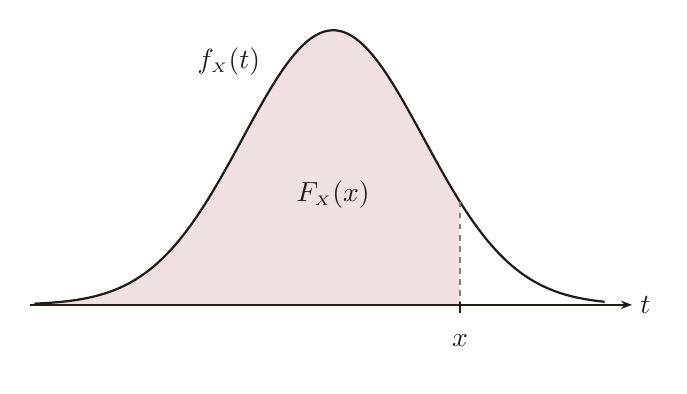
\begin{tikzpicture}[
  x=1.15cm,
  y=8.74cm,
  every node/.style={font=\normalsize, journalink},
  axis/.style={journalink, line width=0.8pt, -{Stealth[length=4pt]}},
  tick/.style={journalink, line width=0.8pt},
  curve/.style={journalink, line width=0.8pt},
  guide/.style={journalmuted, line width=0.5pt, dash pattern=on 2pt off 2pt},
  region/.style={journalaccent, fill opacity=0.15}
]
  % ---- common bounding box, identical in all four figures of this group ----
  \path (-0.43cm,-0.78cm) rectangle (7.58cm,3.52cm);

  % ---- x axis ----
  \draw[axis] (-0.35,0) -- (6.3,0);

  % ---- shaded area: left edge of the drawing up to the threshold x = 4.4 ----
  \fill[region]
    (-0.3,0) -- (4.4,0) -- (4.4,0.1497275)
    -- plot[domain=4.4:-0.3, samples=200, smooth]
       (\x,{0.3989423*exp(-(\x-3)*(\x-3)/2)})
    -- cycle;

  % ---- density curve: N(3,1) ----
  \draw[curve] plot[domain=-0.3:6, samples=200, smooth]
    (\x,{0.3989423*exp(-(\x-3)*(\x-3)/2)});

  % ---- threshold at x = 4.4 ----
  \draw[guide] (4.4,0.1497275) -- (4.4,0);
  \draw[tick] ([yshift=0.035cm]4.4,0) -- ([yshift=-0.106cm]4.4,0);
  \node[anchor=north] at ([yshift=-0.25cm]4.4,0) {$x$};

  % ---- labels ----
  \node[anchor=south east, inner sep=0pt] at ([yshift=0.38cm]2.2,0.2896916)
    {$f_{\sssig X}(t)$};
  % Centred on the shaded region as it is at the label's own height, the same
  % rule as continuous-interval-area.tex.  At yshift 1.40cm the height is
  % 1.40/8.74 = 0.16018; the curve exceeds that for x in [1.649, 4.351], and
  % the threshold x = 4.4 falls outside that span, so at this height both
  % edges of the region are the curve itself and the slice is centred on the
  % mode, x = 3.  (was 2.5, which reads well left of centre.)
  \node[inner sep=0pt] at ([yshift=1.40cm]3.0,0) {$F_{\sssig X}(x)$};
  \node[anchor=west, inner sep=2.8pt] at (6.3,0) {$t$};
\end{tikzpicture}
\end{document}
